\RequirePackage[l2tabu,orthodox]{nag}

% TODO: decide if one-sided/two-sided
%\documentclass[headsepline,footsepline,footinclude=false,fontsize=11pt,paper=a4,listof=totoc,bibliography=totoc,BCOR=12mm,DIV=12]{scrbook} % two-sided % original source stated: BCOR=12mm,DIV=12
\documentclass[headsepline,footsepline,footinclude=false,oneside,fontsize=11pt,paper=a4,listof=totoc,bibliography=totoc,DIV=12]{scrbook} % one-sided

% TODO: change citation style in settings
\PassOptionsToPackage{table,svgnames,dvipsnames}{xcolor}

\usepackage[utf8]{inputenc}
\usepackage[T1]{fontenc}
\usepackage[sc]{mathpazo}
\usepackage[autostyle]{csquotes}
\usepackage[%
  backend=biber,
  url=false,
  style=alphabetic,
  maxnames=4,
  minnames=3,
  maxbibnames=99,
  giveninits,
  uniquename=init]{biblatex} % TODO: adapt citation style
\usepackage{graphicx}
\usepackage{scrhack} % necessary for listings package
\usepackage{listings}
\usepackage{lstautogobble}
\usepackage{tikz}
\usepackage{pgfplots}
\usepackage{pgfplotstable}
\usepackage{booktabs}
\usepackage[final]{microtype}
\usepackage{caption}
\usepackage[hidelinks]{hyperref} % hidelinks removes colored boxes around references and links

\usepackage{amssymb}
\usepackage{amsmath}
\usepackage{amsthm}
\usepackage{float}

\bibliography{bibliography}

\setkomafont{disposition}{\normalfont\bfseries} % use serif font for headings
\linespread{1.05} % adjust line spread for mathpazo font

% Add table of contents to PDF bookmarks
\BeforeTOCHead[toc]{{\cleardoublepage\pdfbookmark[0]{\contentsname}{toc}}}

% Define TUM corporate design colors
% Taken from http://portal.mytum.de/corporatedesign/index_print/vorlagen/index_farben
\definecolor{TUMBlue}{HTML}{0065BD}
\definecolor{TUMSecondaryBlue}{HTML}{005293}
\definecolor{TUMSecondaryBlue2}{HTML}{003359}
\definecolor{TUMBlack}{HTML}{000000}
\definecolor{TUMWhite}{HTML}{FFFFFF}
\definecolor{TUMDarkGray}{HTML}{333333}
\definecolor{TUMGray}{HTML}{808080}
\definecolor{TUMLightGray}{HTML}{CCCCC6}
\definecolor{TUMAccentGray}{HTML}{DAD7CB}
\definecolor{TUMAccentOrange}{HTML}{E37222}
\definecolor{TUMAccentGreen}{HTML}{A2AD00}
\definecolor{TUMAccentLightBlue}{HTML}{98C6EA}
\definecolor{TUMAccentBlue}{HTML}{64A0C8}

% Settings for pgfplots
\pgfplotsset{compat=newest}
\pgfplotsset{
  % For available color names, see http://www.latextemplates.com/svgnames-colors
  cycle list={TUMBlue\\TUMAccentOrange\\TUMAccentGreen\\TUMSecondaryBlue2\\TUMDarkGray\\},
}

% Settings for lstlistings
\lstset{%
  basicstyle=\ttfamily,
  columns=fullflexible,
  autogobble,
  keywordstyle=\bfseries\color{TUMBlue},
  stringstyle=\color{TUMAccentGreen}
}

\definecolor{TUMBlue}{HTML}{0065BD}
\definecolor{TUMSecondaryBlue}{HTML}{005293}
\definecolor{TUMSecondaryBlue2}{HTML}{003359}
\definecolor{TUMBlack}{HTML}{000000}
\definecolor{TUMWhite}{HTML}{FFFFFF}
\definecolor{TUMDarkGray}{HTML}{333333}
\definecolor{TUMGray}{HTML}{808080}
\definecolor{TUMLightGray}{HTML}{CCCCC6}
\definecolor{TUMAccentGray}{HTML}{DAD7CB}
\definecolor{TUMAccentOrange}{HTML}{E37222}
\definecolor{TUMAccentGreen}{HTML}{A2AD00}
\definecolor{TUMAccentLightBlue}{HTML}{98C6EA}
\definecolor{TUMAccentBlue}{HTML}{64A0C8}

% Settings for pgfplots
\pgfplotsset{compat=newest}
\pgfplotsset{
  % For available color names, see http://www.latextemplates.com/svgnames-colors
  cycle list={TUMBlue\\TUMAccentOrange\\TUMAccentGreen\\TUMSecondaryBlue2\\TUMDarkGray\\},
}
\usepackage{ifthen}
\usepackage{/home/zixuan/Isabelle2022_linux/Isabelle2022/lib/texinputs/isabelle}
\usepackage{/home/zixuan/Isabelle2022_linux/Isabelle2022/lib/texinputs/isabellesym}
\isabellestyle{tt}
 
\newcommand{\DefineSnippet}[2]{%
  \expandafter\newcommand\csname snippet--#1\endcsname{%
    \begin{quote}
    \begin{isabelle}
    #2
    \end{isabelle}
    \end{quote}}}
\newcommand{\Snippet}[1]{%
  \ifcsname snippet--#1\endcsname{\csname snippet--#1\endcsname}%
  \else+++++++ERROR: Snippet ``#1 not defined+++++++ \fi}

\DefineSnippet{cnf-sat-def}{
    %
\begin{isabelle}%
    \isacommand{datatype}\isamarkupfalse%
\ {\isacharprime}{\kern0pt}a\ lit\ {\isacharequal}{\kern0pt}\ Pos\ {\isacharprime}{\kern0pt}a\ {\isacharbar}{\kern0pt}\ Neg\ {\isacharprime}{\kern0pt}a\isanewline
\isanewline
\isacommand{type{\isacharunderscore}{\kern0pt}synonym}\isamarkupfalse%
\ {\isacharprime}{\kern0pt}a\ three{\isacharunderscore}{\kern0pt}sat\ {\isacharequal}{\kern0pt}\ {\isachardoublequoteopen}{\isacharprime}{\kern0pt}a\ lit\ set\ list{\isachardoublequoteclose}\isanewline
\isanewline
\isacommand{definition}\isamarkupfalse%
\ lift\ {\isacharcolon}{\kern0pt}{\isacharcolon}{\kern0pt}\ {\isachardoublequoteopen}{\isacharparenleft}{\kern0pt}{\isacharprime}{\kern0pt}a\ {\isasymRightarrow}\ bool{\isacharparenright}{\kern0pt}\ {\isasymRightarrow}\ {\isacharprime}{\kern0pt}a\ lit\ {\isasymRightarrow}\ bool{\isachardoublequoteclose}\ {\isacharparenleft}{\kern0pt}{\isachardoublequoteopen}{\isacharunderscore}{\kern0pt}{\isasymup}{\isachardoublequoteclose}\ {\isadigit{6}}{\isadigit{0}}{\isacharparenright}{\kern0pt}\ \isakeyword{where}\isanewline
\ \ {\isachardoublequoteopen}lift\ {\isasymsigma}\ {\isasymequiv}\ {\isasymlambda}l{\isachardot}{\kern0pt}\ case\ l\ of\ Pos\ x\ {\isasymRightarrow}\ {\isasymsigma}\ x\ {\isacharbar}{\kern0pt}\ Neg\ x\ {\isasymRightarrow}\ {\isasymnot}\ {\isasymsigma}\ x{\isachardoublequoteclose}\isanewline
\isanewline
\isacommand{definition}\isamarkupfalse%
\ models\ {\isacharcolon}{\kern0pt}{\isacharcolon}{\kern0pt}\ {\isachardoublequoteopen}{\isacharparenleft}{\kern0pt}{\isacharprime}{\kern0pt}a\ {\isasymRightarrow}\ bool{\isacharparenright}{\kern0pt}\ {\isasymRightarrow}\ {\isacharprime}{\kern0pt}a\ three{\isacharunderscore}{\kern0pt}sat\ {\isasymRightarrow}\ bool{\isachardoublequoteclose}\ {\isacharparenleft}{\kern0pt}\isakeyword{infixl}\ {\isachardoublequoteopen}{\isasymTurnstile}{\isachardoublequoteclose}\ {\isadigit{5}}{\isadigit{5}}{\isacharparenright}{\kern0pt}\ \isakeyword{where}\isanewline
\ \ {\isachardoublequoteopen}{\isasymsigma}\ {\isasymTurnstile}\ F\ {\isasymequiv}\ {\isasymforall}cls\ {\isasymin}\ set\ F{\isachardot}{\kern0pt}\ {\isasymexists}l\ {\isasymin}\ cls{\isachardot}{\kern0pt}\ {\isacharparenleft}{\kern0pt}{\isasymsigma}{\isasymup}{\isacharparenright}{\kern0pt}\ l{\isachardoublequoteclose}\isanewline
\isanewline
\isacommand{definition}\isamarkupfalse%
\ sat\ {\isacharcolon}{\kern0pt}{\isacharcolon}{\kern0pt}\ {\isachardoublequoteopen}{\isacharprime}{\kern0pt}a\ three{\isacharunderscore}{\kern0pt}sat\ {\isasymRightarrow}\ bool{\isachardoublequoteclose}\ \isakeyword{where}\isanewline
\ \ {\isachardoublequoteopen}sat\ F\ {\isasymequiv}\ {\isasymexists}{\isasymsigma}{\isachardot}{\kern0pt}\ {\isasymsigma}\ {\isasymTurnstile}\ F{\isachardoublequoteclose}\isanewline
\isanewline
\isacommand{definition}\isamarkupfalse%
     {\isachardoublequoteopen}cnf{\isacharunderscore}{\kern0pt}sat\ {\isasymequiv}\ 
     {\isacharbraceleft}{\kern0pt}F{\isachardot}{\kern0pt}\ sat\ F\ {\isasymand}\ 
     {\isacharparenleft}{\kern0pt}{\isasymforall}cls\ {\isasymin}\ set\ F{\isachardot}{\kern0pt}\ 
     finite\ cls{\isacharparenright}{\kern0pt}{\isacharbraceright}{\kern0pt}{\isachardoublequoteclose}%
\end{isabelle}
}

\DefineSnippet{exact-cover-def}{
    \isacommand{definition}\isamarkupfalse%
\ {\isachardoublequoteopen}exact{\isacharunderscore}{\kern0pt}cover\ {\isasymequiv}\ {\isacharbraceleft}{\kern0pt}{\isacharparenleft}{\kern0pt}X{\isacharcomma}{\kern0pt}\ S{\isacharparenright}{\kern0pt}{\isachardot}{\kern0pt}\ finite\ X\ {\isasymand}\ {\isasymUnion}S\ {\isasymsubseteq}\ X\ {\isasymand}\ {\isacharparenleft}{\kern0pt}{\isasymexists}S{\isacharprime}{\kern0pt}\ {\isasymsubseteq}\ S{\isachardot}{\kern0pt}\ {\isasymUnion}S{\isacharprime}{\kern0pt}\ {\isacharequal}{\kern0pt}\ X\ {\isasymand}\ disjoint\ S{\isacharprime}{\kern0pt}{\isacharparenright}{\kern0pt}{\isacharbraceright}{\kern0pt}{\isachardoublequoteclose}

}

\DefineSnippet{exact-cover-basics}{
    \isacommand{datatype}\isamarkupfalse%
\ {\isacharprime}{\kern0pt}a\ xc{\isacharunderscore}{\kern0pt}element\ {\isacharequal}{\kern0pt}\ V\ {\isacharprime}{\kern0pt}a\ {\isacharbar}{\kern0pt}\ C\ {\isachardoublequoteopen}{\isacharprime}{\kern0pt}a\ lit\ set{\isachardoublequoteclose}\ {\isacharbar}{\kern0pt}\ L\ {\isachardoublequoteopen}{\isacharprime}{\kern0pt}a\ lit{\isachardoublequoteclose}\ {\isachardoublequoteopen}{\isacharprime}{\kern0pt}a\ lit\ set{\isachardoublequoteclose}\isanewline
\isanewline
\isacommand{fun}\isamarkupfalse%
\ var\ {\isacharcolon}{\kern0pt}{\isacharcolon}{\kern0pt}\ {\isachardoublequoteopen}{\isacharprime}{\kern0pt}a\ lit\ {\isasymRightarrow}\ {\isacharprime}{\kern0pt}a{\isachardoublequoteclose}\ \isakeyword{where}\ \isanewline
{\isachardoublequoteopen}var\ {\isacharparenleft}{\kern0pt}Neg\ a{\isacharparenright}{\kern0pt}\ {\isacharequal}{\kern0pt}\ a{\isachardoublequoteclose}\ {\isacharbar}{\kern0pt}\ {\isachardoublequoteopen}var\ {\isacharparenleft}{\kern0pt}Pos\ a{\isacharparenright}{\kern0pt}\ {\isacharequal}{\kern0pt}\ a{\isachardoublequoteclose}\isanewline
\isanewline
\isacommand{definition}\isamarkupfalse%
\ {\isachardoublequoteopen}vars\ F\ {\isasymequiv}\ {\isacharparenleft}{\kern0pt}var{\isacharparenright}{\kern0pt}\ {\isacharbackquote}{\kern0pt}\ {\isasymUnion}\ {\isacharparenleft}{\kern0pt}set\ F{\isacharparenright}{\kern0pt}{\isachardoublequoteclose}\isanewline
\isanewline
\isacommand{definition}\isamarkupfalse%
\ vars{\isacharunderscore}{\kern0pt}of{\isacharunderscore}{\kern0pt}sat\ {\isacharcolon}{\kern0pt}{\isacharcolon}{\kern0pt}\ {\isachardoublequoteopen}{\isacharprime}{\kern0pt}a\ three{\isacharunderscore}{\kern0pt}sat\ {\isasymRightarrow}\ {\isacharprime}{\kern0pt}a\ xc{\isacharunderscore}{\kern0pt}element\ set{\isachardoublequoteclose}\ \isakeyword{where}\isanewline
\ \ {\isachardoublequoteopen}vars{\isacharunderscore}{\kern0pt}of{\isacharunderscore}{\kern0pt}sat\ F\ {\isacharequal}{\kern0pt}\ {\isacharbraceleft}{\kern0pt}V\ v\ {\isacharbar}{\kern0pt}v{\isachardot}{\kern0pt}\ v\ {\isasymin}\ vars\ F{\isacharbraceright}{\kern0pt}{\isachardoublequoteclose}\isanewline
\isanewline
\isacommand{definition}\isamarkupfalse%
\ clauses{\isacharunderscore}{\kern0pt}of{\isacharunderscore}{\kern0pt}sat\ {\isacharcolon}{\kern0pt}{\isacharcolon}{\kern0pt}\ {\isachardoublequoteopen}{\isacharprime}{\kern0pt}a\ three{\isacharunderscore}{\kern0pt}sat\ {\isasymRightarrow}\ {\isacharprime}{\kern0pt}a\ xc{\isacharunderscore}{\kern0pt}element\ set{\isachardoublequoteclose}\ \isakeyword{where}\ \isanewline
\ \ {\isachardoublequoteopen}clauses{\isacharunderscore}{\kern0pt}of{\isacharunderscore}{\kern0pt}sat\ F\ {\isacharequal}{\kern0pt}\ {\isacharbraceleft}{\kern0pt}C\ c{\isacharbar}{\kern0pt}\ c{\isachardot}{\kern0pt}\ c{\isasymin}\ set\ F{\isacharbraceright}{\kern0pt}{\isachardoublequoteclose}\isanewline
\isanewline
\isacommand{definition}\isamarkupfalse%
\ literals{\isacharunderscore}{\kern0pt}of{\isacharunderscore}{\kern0pt}sat\ {\isacharcolon}{\kern0pt}{\isacharcolon}{\kern0pt}\ {\isachardoublequoteopen}{\isacharprime}{\kern0pt}a\ three{\isacharunderscore}{\kern0pt}sat\ {\isasymRightarrow}\ {\isacharprime}{\kern0pt}a\ xc{\isacharunderscore}{\kern0pt}element\ set{\isachardoublequoteclose}\ \isakeyword{where}\isanewline
{\isachardoublequoteopen}literals{\isacharunderscore}{\kern0pt}of{\isacharunderscore}{\kern0pt}sat\ F\ {\isacharequal}{\kern0pt}\ {\isacharbraceleft}{\kern0pt}L\ l\ c{\isacharbar}{\kern0pt}\ l\ c{\isachardot}{\kern0pt}\ c\ {\isasymin}\ set\ F\ {\isasymand}\ l\ {\isasymin}\ c{\isacharbraceright}{\kern0pt}{\isachardoublequoteclose}
}

\DefineSnippet{exact-cover-red}{
    \isacommand{definition}\isamarkupfalse%
\ literal{\isacharunderscore}{\kern0pt}sets\isanewline
\ \ {\isacharcolon}{\kern0pt}{\isacharcolon}{\kern0pt}\ {\isachardoublequoteopen}{\isacharprime}{\kern0pt}a\ three{\isacharunderscore}{\kern0pt}sat\ \ {\isasymRightarrow}\ {\isacharprime}{\kern0pt}a\ xc{\isacharunderscore}{\kern0pt}element\ set\ set{\isachardoublequoteclose}\ \isakeyword{where}\isanewline
{\isachardoublequoteopen}literal{\isacharunderscore}{\kern0pt}sets\ F\ {\isacharequal}{\kern0pt}\ {\isacharbraceleft}{\kern0pt}{\isacharbraceleft}{\kern0pt}l{\isacharbraceright}{\kern0pt}{\isacharbar}{\kern0pt}\ l{\isachardot}{\kern0pt}\ l\ {\isasymin}\ {\isacharparenleft}{\kern0pt}literals{\isacharunderscore}{\kern0pt}of{\isacharunderscore}{\kern0pt}sat\ F{\isacharparenright}{\kern0pt}{\isacharbraceright}{\kern0pt}{\isachardoublequoteclose}\isanewline
\isanewline
\isacommand{definition}\isamarkupfalse%
\ clauses{\isacharunderscore}{\kern0pt}with{\isacharunderscore}{\kern0pt}literals\ \isanewline
\ \ {\isacharcolon}{\kern0pt}{\isacharcolon}{\kern0pt}\ {\isachardoublequoteopen}{\isacharprime}{\kern0pt}a\ three{\isacharunderscore}{\kern0pt}sat\ {\isasymRightarrow}\ {\isacharprime}{\kern0pt}a\ xc{\isacharunderscore}{\kern0pt}element\ set\ set{\isachardoublequoteclose}\ \isakeyword{where}\isanewline
{\isachardoublequoteopen}clauses{\isacharunderscore}{\kern0pt}with{\isacharunderscore}{\kern0pt}literals\ F\ {\isacharequal}{\kern0pt}\ {\isacharbraceleft}{\kern0pt}{\isacharbraceleft}{\kern0pt}C\ c{\isacharcomma}{\kern0pt}\ l{\isacharbraceright}{\kern0pt}\ {\isacharbar}{\kern0pt}c\ l{\isachardot}{\kern0pt}\ C\ c\ {\isasymin}\ {\isacharparenleft}{\kern0pt}clauses{\isacharunderscore}{\kern0pt}of{\isacharunderscore}{\kern0pt}sat\ F{\isacharparenright}{\kern0pt}\ {\isasymand}\ l\ {\isasymin}\ {\isacharparenleft}{\kern0pt}literals{\isacharunderscore}{\kern0pt}of{\isacharunderscore}{\kern0pt}sat\ F{\isacharparenright}{\kern0pt}\ \isanewline
\ \ \ \ \ \ \ \ {\isasymand}\ l\ {\isasymin}\ {\isacharbraceleft}{\kern0pt}L\ a\ c\ {\isacharbar}{\kern0pt}\ a{\isachardot}{\kern0pt}\ a\ {\isasymin}\ c{\isacharbraceright}{\kern0pt}{\isacharbraceright}{\kern0pt}{\isachardoublequoteclose}\isanewline
\isanewline
\isacommand{definition}\isamarkupfalse%
\ var{\isacharunderscore}{\kern0pt}true{\isacharunderscore}{\kern0pt}literals\isanewline
\ \ {\isacharcolon}{\kern0pt}{\isacharcolon}{\kern0pt}\ {\isachardoublequoteopen}{\isacharprime}{\kern0pt}a\ three{\isacharunderscore}{\kern0pt}sat\ {\isasymRightarrow}\ {\isacharprime}{\kern0pt}a\ xc{\isacharunderscore}{\kern0pt}element\ set\ set{\isachardoublequoteclose}\ \isakeyword{where}\ \isanewline
{\isachardoublequoteopen}var{\isacharunderscore}{\kern0pt}true{\isacharunderscore}{\kern0pt}literals\ F\ {\isacharequal}{\kern0pt}\ \isanewline
\ \ {\isacharbraceleft}{\kern0pt}{\isacharbraceleft}{\kern0pt}V\ v{\isacharbraceright}{\kern0pt}\ {\isasymunion}\ {\isacharbraceleft}{\kern0pt}l{\isachardot}{\kern0pt}\ l\ {\isasymin}\ {\isacharparenleft}{\kern0pt}literals{\isacharunderscore}{\kern0pt}of{\isacharunderscore}{\kern0pt}sat\ F{\isacharparenright}{\kern0pt}\ \isanewline
\ \ {\isasymand}\ {\isacharparenleft}{\kern0pt}{\isasymexists}c{\isachardot}{\kern0pt}\ C\ c{\isasymin}\ {\isacharparenleft}{\kern0pt}clauses{\isacharunderscore}{\kern0pt}of{\isacharunderscore}{\kern0pt}sat\ F{\isacharparenright}{\kern0pt}\ {\isasymand}\ L\ {\isacharparenleft}{\kern0pt}Neg\ v{\isacharparenright}{\kern0pt}\ c\ {\isacharequal}{\kern0pt}\ l{\isacharparenright}{\kern0pt}{\isacharbraceright}{\kern0pt}\ {\isacharbar}{\kern0pt}v{\isachardot}{\kern0pt}\ V\ v\ {\isasymin}\ {\isacharparenleft}{\kern0pt}vars{\isacharunderscore}{\kern0pt}of{\isacharunderscore}{\kern0pt}sat\ F{\isacharparenright}{\kern0pt}{\isacharbraceright}{\kern0pt}{\isachardoublequoteclose}\isanewline
\isanewline
\isacommand{definition}\isamarkupfalse%
\ var{\isacharunderscore}{\kern0pt}false{\isacharunderscore}{\kern0pt}literals\isanewline
\ \ \ \ {\isacharcolon}{\kern0pt}{\isacharcolon}{\kern0pt}\ {\isachardoublequoteopen}{\isacharprime}{\kern0pt}a\ three{\isacharunderscore}{\kern0pt}sat\ {\isasymRightarrow}\ {\isacharprime}{\kern0pt}a\ xc{\isacharunderscore}{\kern0pt}element\ set\ set{\isachardoublequoteclose}\ \isakeyword{where}\ \isanewline
{\isachardoublequoteopen}var{\isacharunderscore}{\kern0pt}false{\isacharunderscore}{\kern0pt}literals\ F\ {\isacharequal}{\kern0pt}\ \isanewline
\ \ {\isacharbraceleft}{\kern0pt}{\isacharbraceleft}{\kern0pt}V\ v{\isacharbraceright}{\kern0pt}\ {\isasymunion}\ {\isacharbraceleft}{\kern0pt}l{\isachardot}{\kern0pt}\ l\ {\isasymin}\ {\isacharparenleft}{\kern0pt}literals{\isacharunderscore}{\kern0pt}of{\isacharunderscore}{\kern0pt}sat\ F{\isacharparenright}{\kern0pt}\ \isanewline
\ \ {\isasymand}\ {\isacharparenleft}{\kern0pt}{\isasymexists}c{\isachardot}{\kern0pt}\ C\ c{\isasymin}\ {\isacharparenleft}{\kern0pt}clauses{\isacharunderscore}{\kern0pt}of{\isacharunderscore}{\kern0pt}sat\ F{\isacharparenright}{\kern0pt}\ {\isasymand}\ L\ {\isacharparenleft}{\kern0pt}Pos\ v{\isacharparenright}{\kern0pt}\ c\ {\isacharequal}{\kern0pt}\ l{\isacharparenright}{\kern0pt}{\isacharbraceright}{\kern0pt}\ {\isacharbar}{\kern0pt}v{\isachardot}{\kern0pt}\ V\ v\ {\isasymin}\ {\isacharparenleft}{\kern0pt}vars{\isacharunderscore}{\kern0pt}of{\isacharunderscore}{\kern0pt}sat\ F{\isacharparenright}{\kern0pt}{\isacharbraceright}{\kern0pt}{\isachardoublequoteclose}\isanewline
\isanewline
\isacommand{abbreviation}\isamarkupfalse%
\ {\isachardoublequoteopen}comp{\isacharunderscore}{\kern0pt}X\ F\ {\isasymequiv}\ \isanewline
\ \ vars{\isacharunderscore}{\kern0pt}of{\isacharunderscore}{\kern0pt}sat\ F\ {\isasymunion}\ clauses{\isacharunderscore}{\kern0pt}of{\isacharunderscore}{\kern0pt}sat\ F\ {\isasymunion}\ literals{\isacharunderscore}{\kern0pt}of{\isacharunderscore}{\kern0pt}sat\ F{\isachardoublequoteclose}\isanewline
\isacommand{abbreviation}\isamarkupfalse%
\ {\isachardoublequoteopen}comp{\isacharunderscore}{\kern0pt}S\ F\ {\isasymequiv}\ \isanewline
\ \ \ \ literal{\isacharunderscore}{\kern0pt}sets\ F\ {\isasymunion}\ clauses{\isacharunderscore}{\kern0pt}with{\isacharunderscore}{\kern0pt}literals\ F\ \isanewline
\ \ {\isasymunion}\ var{\isacharunderscore}{\kern0pt}true{\isacharunderscore}{\kern0pt}literals\ F\ {\isasymunion}\ var{\isacharunderscore}{\kern0pt}false{\isacharunderscore}{\kern0pt}literals\ F{\isachardoublequoteclose}\isanewline
\isanewline
\isacommand{definition}\isamarkupfalse%
\ sat{\isacharunderscore}{\kern0pt}xc\ {\isacharcolon}{\kern0pt}{\isacharcolon}{\kern0pt}\ {\isachardoublequoteopen}{\isacharprime}{\kern0pt}a\ three{\isacharunderscore}{\kern0pt}sat\ {\isasymRightarrow}\ {\isacharprime}{\kern0pt}a\ xc{\isacharunderscore}{\kern0pt}element\ set\ {\isacharasterisk}{\kern0pt}\ {\isacharprime}{\kern0pt}a\ xc{\isacharunderscore}{\kern0pt}element\ set\ set{\isachardoublequoteclose}\ \isakeyword{where}\ \isanewline
{\isachardoublequoteopen}sat{\isacharunderscore}{\kern0pt}xc\ F\ {\isacharequal}{\kern0pt}\ {\isacharparenleft}{\kern0pt}comp{\isacharunderscore}{\kern0pt}X\ F{\isacharcomma}{\kern0pt}\ comp{\isacharunderscore}{\kern0pt}S\ F{\isacharparenright}{\kern0pt}{\isachardoublequoteclose}
}

\DefineSnippet{exact-cover-prf}{
    \isacommand{definition}\isamarkupfalse%
\ constr{\isacharunderscore}{\kern0pt}cover{\isacharunderscore}{\kern0pt}clause\isanewline
\ \ {\isacharcolon}{\kern0pt}{\isacharcolon}{\kern0pt}\ {\isachardoublequoteopen}{\isacharprime}{\kern0pt}a\ lit\ set\ {\isasymRightarrow}\ {\isacharparenleft}{\kern0pt}{\isacharprime}{\kern0pt}a\ {\isasymRightarrow}\ bool{\isacharparenright}{\kern0pt}\ {\isasymRightarrow}\ {\isacharprime}{\kern0pt}a\ xc{\isacharunderscore}{\kern0pt}element\ set\ set{\isachardoublequoteclose}\ \isakeyword{where}\ \isanewline
{\isachardoublequoteopen}constr{\isacharunderscore}{\kern0pt}cover{\isacharunderscore}{\kern0pt}clause\ c\ {\isasymsigma}\ {\isacharequal}{\kern0pt}\ \isanewline
\ \ {\isacharparenleft}{\kern0pt}SOME\ s{\isachardot}{\kern0pt}\ {\isasymexists}p\ {\isasymin}\ c{\isachardot}{\kern0pt}\ {\isacharparenleft}{\kern0pt}{\isasymsigma}{\isasymup}{\isacharparenright}{\kern0pt}\ p\ {\isasymand}\ s\ {\isacharequal}{\kern0pt}\ {\isacharbraceleft}{\kern0pt}{\isacharbraceleft}{\kern0pt}C\ c{\isacharcomma}{\kern0pt}\ L\ p\ c{\isacharbraceright}{\kern0pt}{\isacharbraceright}{\kern0pt}\ {\isasymunion}\ {\isacharbraceleft}{\kern0pt}{\isacharbraceleft}{\kern0pt}L\ q\ c{\isacharbraceright}{\kern0pt}\ {\isacharbar}{\kern0pt}\ q{\isachardot}{\kern0pt}\ q\ {\isasymin}\ c\ {\isasymand}\ q\ {\isasymnoteq}\ p\ {\isasymand}\ {\isacharparenleft}{\kern0pt}{\isasymsigma}{\isasymup}{\isacharparenright}{\kern0pt}\ q{\isacharbraceright}{\kern0pt}{\isacharparenright}{\kern0pt}{\isachardoublequoteclose}\ \isanewline
\isanewline
\isacommand{lemma}\isamarkupfalse%
\ constr{\isacharunderscore}{\kern0pt}cover{\isacharunderscore}{\kern0pt}clause{\isacharunderscore}{\kern0pt}unfold{\isacharcolon}{\kern0pt}\isanewline
\isakeyword{assumes}\ {\isachardoublequoteopen}{\isasymsigma}\ {\isasymTurnstile}\ F{\isachardoublequoteclose}\ {\isachardoublequoteopen}c\ {\isasymin}\ set\ F{\isachardoublequoteclose}\isanewline
\isakeyword{shows}\ {\isachardoublequoteopen}{\isasymexists}p{\isasymin}c{\isachardot}{\kern0pt}\ {\isacharparenleft}{\kern0pt}{\isasymsigma}{\isasymup}{\isacharparenright}{\kern0pt}\ p\ {\isasymand}\ constr{\isacharunderscore}{\kern0pt}cover{\isacharunderscore}{\kern0pt}clause\ c\ {\isasymsigma}\ {\isacharequal}{\kern0pt}\ {\isacharbraceleft}{\kern0pt}{\isacharbraceleft}{\kern0pt}C\ c{\isacharcomma}{\kern0pt}\ L\ p\ c{\isacharbraceright}{\kern0pt}{\isacharbraceright}{\kern0pt}\ {\isasymunion}\ {\isacharbraceleft}{\kern0pt}{\isacharbraceleft}{\kern0pt}L\ q\ c{\isacharbraceright}{\kern0pt}\ {\isacharbar}{\kern0pt}\ q{\isachardot}{\kern0pt}\ q\ {\isasymin}\ c\ {\isasymand}\ q\ {\isasymnoteq}\ p\ {\isasymand}\ {\isacharparenleft}{\kern0pt}{\isasymsigma}{\isasymup}{\isacharparenright}{\kern0pt}\ q{\isacharbraceright}{\kern0pt}{\isachardoublequoteclose}
}

\DefineSnippet{exact-cover-correct}{
    \isacommand{lemma}\isamarkupfalse%
\ sat{\isacharunderscore}{\kern0pt}xc{\isacharunderscore}{\kern0pt}complete{\isacharcolon}{\kern0pt}\isanewline
\ \ {\isachardoublequoteopen}sat{\isacharunderscore}{\kern0pt}xc\ F\ {\isasymin}\ exact{\isacharunderscore}{\kern0pt}cover\ {\isasymLongrightarrow}\ F\ {\isasymin}\ cnf{\isacharunderscore}{\kern0pt}sat{\isachardoublequoteclose}
\isanewline \isanewline 
\isacommand{lemma}\isamarkupfalse%
\ sat{\isacharunderscore}{\kern0pt}xc{\isacharunderscore}{\kern0pt}sound{\isacharcolon}{\kern0pt}\isanewline
\ \ {\isachardoublequoteopen}F\ {\isasymin}\ cnf{\isacharunderscore}{\kern0pt}sat\ {\isasymLongrightarrow}\ sat{\isacharunderscore}{\kern0pt}xc\ F\ {\isasymin}\ exact{\isacharunderscore}{\kern0pt}cover{\isachardoublequoteclose}
\isanewline \isanewline 
\isacommand{theorem}\isamarkupfalse%
\ is{\isacharunderscore}{\kern0pt}reduction{\isacharunderscore}{\kern0pt}sat{\isacharunderscore}{\kern0pt}xc{\isacharcolon}{\kern0pt}\isanewline
{\isachardoublequoteopen}is{\isacharunderscore}{\kern0pt}reduction\ sat{\isacharunderscore}{\kern0pt}xc\ cnf{\isacharunderscore}{\kern0pt}sat\ exact{\isacharunderscore}{\kern0pt}cover{\isachardoublequoteclose}
}

\DefineSnippet{exact-cover-poly}{
    \isacommand{definition}\isamarkupfalse%
\ {\isachardoublequoteopen}sat{\isacharunderscore}{\kern0pt}to{\isacharunderscore}{\kern0pt}xc{\isacharunderscore}{\kern0pt}alg{\kern0pt}\ {\isasymequiv}\ {\isacharparenleft}{\kern0pt}{\isasymlambda}F{\isachardot}{\kern0pt}\isanewline
\ do\ \isanewline
\ \ \ \ {\isacharbraceleft}{\kern0pt}\isanewline
\ \ \ \ \ \ VS\ {\isasymleftarrow}\ mop{\isacharunderscore}{\kern0pt}vars{\isacharunderscore}{\kern0pt}of{\isacharunderscore}{\kern0pt}sat\ F{\isacharsemicolon}{\kern0pt}\isanewline
\ \ \ \ \ \ CS\ {\isasymleftarrow}\ mop{\isacharunderscore}{\kern0pt}clauses{\isacharunderscore}{\kern0pt}of{\isacharunderscore}{\kern0pt}sat\ F{\isacharsemicolon}{\kern0pt}\isanewline
\ \ \ \ \ \ LS\ {\isasymleftarrow}\ mop{\isacharunderscore}{\kern0pt}literals{\isacharunderscore}{\kern0pt}of{\isacharunderscore}{\kern0pt}sat\ F{\isacharsemicolon}{\kern0pt}\isanewline
\ \ \ \ \ \ s{\isadigit{1}}\ {\isasymleftarrow}\ mop{\isacharunderscore}{\kern0pt}literal{\isacharunderscore}{\kern0pt}sets\ F{\isacharsemicolon}{\kern0pt}\isanewline
\ \ \ \ \ \ s{\isadigit{2}}\ {\isasymleftarrow}\ mop{\isacharunderscore}{\kern0pt}clauses{\isacharunderscore}{\kern0pt}with{\isacharunderscore}{\kern0pt}literals\ F{\isacharsemicolon}{\kern0pt}\isanewline
\ \ \ \ \ \ s{\isadigit{3}}\ {\isasymleftarrow}\ mop{\isacharunderscore}{\kern0pt}var{\isacharunderscore}{\kern0pt}true{\isacharunderscore}{\kern0pt}literals\ F{\isacharsemicolon}{\kern0pt}\isanewline
\ \ \ \ \ \ s{\isadigit{4}}\ {\isasymleftarrow}\ mop{\isacharunderscore}{\kern0pt}var{\isacharunderscore}{\kern0pt}false{\isacharunderscore}{\kern0pt}literals\ F{\isacharsemicolon}{\kern0pt}\isanewline
\ \ \ \ \ \ X\ {\isasymleftarrow}\ mop{\isacharunderscore}{\kern0pt}union{\isacharunderscore}{\kern0pt}x\ CS\ VS\ LS{\isacharsemicolon}{\kern0pt}\isanewline
\ \ \ \ \ \ S\ {\isasymleftarrow}\ mop{\isacharunderscore}{\kern0pt}union{\isacharunderscore}{\kern0pt}s\ s{\isadigit{1}}\ s{\isadigit{2}}\ s{\isadigit{3}}\ s{\isadigit{4}}{\isacharsemicolon}{\kern0pt}\isanewline
\ \ \ \ \ \ RETURNT\ {\isacharparenleft}{\kern0pt}X{\isacharcomma}{\kern0pt}\ S{\isacharparenright}{\kern0pt}\isanewline
\ \ \ \ {\isacharbraceright}{\kern0pt}\isanewline
{\isacharparenright}{\kern0pt}{\isachardoublequoteclose}\isanewline
\isanewline
\isacommand{definition}\isamarkupfalse%
\ {\isachardoublequoteopen}sat{\isacharunderscore}{\kern0pt}to{\isacharunderscore}{\kern0pt}xc{\isacharunderscore}{\kern0pt}time{\isacharunderscore}{\kern0pt}aux{\kern0pt}\ l\ m\ n\ {\isacharequal}{\kern0pt}\ \isanewline
\ \ {\isadigit{2}}\ {\isacharasterisk}{\kern0pt}\ m\ {\isacharplus}{\kern0pt}\ {\isadigit{3}}\ {\isacharasterisk}{\kern0pt}\ n\ {\isacharplus}{\kern0pt}\ {\isadigit{1}}\ {\isacharplus}{\kern0pt}\ {\isadigit{1}}\isanewline
{\isacharplus}{\kern0pt}\ {\isadigit{3}}\ {\isacharasterisk}{\kern0pt}\ l\ {\isacharplus}{\kern0pt}\ {\isadigit{3}}\ {\isacharasterisk}{\kern0pt}\ m\ {\isacharplus}{\kern0pt}\ m\ {\isacharplus}{\kern0pt}\ {\isadigit{3}}\ {\isacharasterisk}{\kern0pt}\ n\isanewline
{\isacharplus}{\kern0pt}\ {\isacharparenleft}{\kern0pt}{\isadigit{3}}\ {\isacharplus}{\kern0pt}\ {\isadigit{1}}{\isacharparenright}{\kern0pt}\ {\isacharasterisk}{\kern0pt}\ n\ {\isacharplus}{\kern0pt}\ {\isacharparenleft}{\kern0pt}{\isadigit{3}}\ {\isacharplus}{\kern0pt}\ {\isadigit{1}}\ {\isacharplus}{\kern0pt}\ {\isadigit{1}}{\isacharparenright}{\kern0pt}\ {\isacharasterisk}{\kern0pt}\ n\ {\isacharplus}{\kern0pt}\ m\isanewline
{\isacharplus}{\kern0pt}\ {\isacharparenleft}{\kern0pt}{\isadigit{3}}\ {\isacharplus}{\kern0pt}\ {\isadigit{1}}{\isacharparenright}{\kern0pt}\ {\isacharasterisk}{\kern0pt}\ l\ {\isacharplus}{\kern0pt}\ {\isacharparenleft}{\kern0pt}{\isadigit{3}}\ {\isacharplus}{\kern0pt}\ {\isadigit{1}}\ {\isacharplus}{\kern0pt}\ {\isadigit{1}}{\isacharparenright}{\kern0pt}\ {\isacharasterisk}{\kern0pt}\ n\ {\isacharplus}{\kern0pt}\ {\isacharparenleft}{\kern0pt}{\isadigit{1}}\ {\isacharplus}{\kern0pt}\ {\isadigit{1}}{\isacharparenright}{\kern0pt}\ {\isacharasterisk}{\kern0pt}\ m\ {\isacharplus}{\kern0pt}\ {\isadigit{1}}\isanewline
{\isacharplus}{\kern0pt}\ {\isacharparenleft}{\kern0pt}{\isadigit{3}}\ {\isacharplus}{\kern0pt}\ {\isadigit{1}}{\isacharparenright}{\kern0pt}\ {\isacharasterisk}{\kern0pt}\ l\ {\isacharplus}{\kern0pt}\ {\isacharparenleft}{\kern0pt}{\isadigit{3}}\ {\isacharplus}{\kern0pt}\ {\isadigit{1}}\ {\isacharplus}{\kern0pt}\ {\isadigit{1}}{\isacharparenright}{\kern0pt}\ {\isacharasterisk}{\kern0pt}\ n\ {\isacharplus}{\kern0pt}\ {\isacharparenleft}{\kern0pt}{\isadigit{1}}\ {\isacharplus}{\kern0pt}\ {\isadigit{1}}{\isacharparenright}{\kern0pt}\ {\isacharasterisk}{\kern0pt}\ m\ {\isacharplus}{\kern0pt}\ {\isadigit{1}}\isanewline
{\isacharplus}{\kern0pt}\ {\isadigit{2}}\ {\isacharplus}{\kern0pt}\ {\isadigit{3}}{\isachardoublequoteclose}\isanewline
\isanewline
\isacommand{definition}\isamarkupfalse%
\ {\isachardoublequoteopen}sat{\isacharunderscore}{\kern0pt}to{\isacharunderscore}{\kern0pt}xc{\isacharunderscore}{\kern0pt}space{\isacharunderscore}{\kern0pt}aux{\kern0pt}\ l\ m\ n\ {\isacharequal}{\kern0pt}\ \isanewline
l\ {\isacharplus}{\kern0pt}\ m\ {\isacharplus}{\kern0pt}\ n\isanewline
{\isacharplus}{\kern0pt}\ n\ {\isacharplus}{\kern0pt}\ n\isanewline
{\isacharplus}{\kern0pt}\ l\ {\isacharplus}{\kern0pt}\ l{\isachardoublequoteclose}
}

\DefineSnippet{exact-cover-polyaux}{
    \isacommand{lemma}\isamarkupfalse%
\ card{\isacharunderscore}{\kern0pt}Un{\isacharunderscore}{\kern0pt}le{\isacharunderscore}{\kern0pt}{\isadigit{4}}{\isacharcolon}{\kern0pt}\isanewline
{\isachardoublequoteopen}card\ {\isacharparenleft}{\kern0pt}a\ {\isasymunion}\ b\ {\isasymunion}\ c\ {\isasymunion}\ d{\isacharparenright}{\kern0pt}\ {\isasymle}\ card\ a\ {\isacharplus}{\kern0pt}\ card\ b\ {\isacharplus}{\kern0pt}\ card\ c\ {\isacharplus}{\kern0pt}\ card\ d{\isachardoublequoteclose}
}

\DefineSnippet{exact-cover-final}{
\isacommand{lemma}\isamarkupfalse%
\ sat{\isacharunderscore}{\kern0pt}to{\isacharunderscore}{\kern0pt}xc{\isacharunderscore}{\kern0pt}size{\isacharcolon}{\kern0pt}\isanewline
{\isachardoublequoteopen}size{\isacharunderscore}{\kern0pt}XC\ {\isacharparenleft}{\kern0pt}sat{\isacharunderscore}{\kern0pt}xc\ F{\isacharparenright}{\kern0pt}\ {\isasymle}\ sat{\isacharunderscore}{\kern0pt}to{\isacharunderscore}{\kern0pt}xc{\isacharunderscore}{\kern0pt}space\ {\isacharparenleft}{\kern0pt}size{\isacharunderscore}{\kern0pt}SAT{\isacharunderscore}{\kern0pt}max\ F{\isacharparenright}{\kern0pt}{\isachardoublequoteclose}\isanewline
\isanewline
\isacommand{lemma}\isamarkupfalse%
\ sat{\isacharunderscore}{\kern0pt}to{\isacharunderscore}{\kern0pt}xc{\isacharunderscore}{\kern0pt}refines{\isacharcolon}{\kern0pt}\isanewline
{\isachardoublequoteopen}sat{\isacharunderscore}{\kern0pt}to{\isacharunderscore}{\kern0pt}xc{\isacharunderscore}{\kern0pt}alg\ F\ {\isasymle}\ \isanewline
\ \ SPEC\ {\isacharparenleft}{\kern0pt}{\isasymlambda}y{\isachardot}{\kern0pt}\ y\ {\isacharequal}{\kern0pt}\ sat{\isacharunderscore}{\kern0pt}xc\ F{\isacharparenright}{\kern0pt}\ {\isacharparenleft}{\kern0pt}{\isasymlambda}{\isacharunderscore}{\kern0pt}{\isachardot}{\kern0pt}\ sat{\isacharunderscore}{\kern0pt}to{\isacharunderscore}{\kern0pt}xc{\isacharunderscore}{\kern0pt}time\ {\isacharparenleft}{\kern0pt}size{\isacharunderscore}{\kern0pt}SAT{\isacharunderscore}{\kern0pt}max\ F{\isacharparenright}{\kern0pt}{\isacharparenright}{\kern0pt}{\isachardoublequoteclose}\isanewline
\isanewline
\isacommand{theorem}\isamarkupfalse%
\ is{\isacharunderscore}{\kern0pt}reduction{\isacharunderscore}{\kern0pt}sat{\isacharunderscore}{\kern0pt}xc{\isacharcolon}{\kern0pt}\isanewline
{\isachardoublequoteopen}is{\isacharunderscore}{\kern0pt}reduction\ sat{\isacharunderscore}{\kern0pt}xc\ cnf{\isacharunderscore}{\kern0pt}sat\ exact{\isacharunderscore}{\kern0pt}cover{\isachardoublequoteclose}

}

\DefineSnippet{exact-hitting-set-def}{
    \isacommand{definition}\isamarkupfalse%
\ {\isachardoublequoteopen}exact{\isacharunderscore}{\kern0pt}hitting{\isacharunderscore}{\kern0pt}set\ {\isasymequiv}\ {\isacharbraceleft}{\kern0pt}S{\isachardot}{\kern0pt}\ {\isasymexists}W{\isachardot}{\kern0pt}\ finite\ W\ {\isasymand}\ {\isacharparenleft}{\kern0pt}{\isasymforall}s\ {\isasymin}\ S{\isachardot}{\kern0pt}\ card\ {\isacharparenleft}{\kern0pt}W\ {\isasyminter}\ s{\isacharparenright}{\kern0pt}\ {\isacharequal}{\kern0pt}\ {\isadigit{1}}{\isacharparenright}{\kern0pt}{\isacharbraceright}{\kern0pt}{\isachardoublequoteclose}
}

\DefineSnippet{exact-hitting-set-reduction}{
\isacommand{definition}\isamarkupfalse%
\ {\isachardoublequoteopen}xc{\isacharunderscore}{\kern0pt}to{\isacharunderscore}{\kern0pt}ehs\ {\isasymequiv}\ {\isasymlambda}{\isacharparenleft}{\kern0pt}X{\isacharcomma}{\kern0pt}\ S{\isacharparenright}{\kern0pt}{\isachardot}{\kern0pt}\ {\isacharparenleft}{\kern0pt}if\ finite\ X\ {\isasymand}\ {\isasymUnion}S\ {\isasymsubseteq}\ X\ then\ {\isacharbraceleft}{\kern0pt}{\isacharbraceleft}{\kern0pt}s{\isachardot}{\kern0pt}\ u\ {\isasymin}\ s\ {\isasymand}\ s\ {\isasymin}\ S{\isacharbraceright}{\kern0pt}\ {\isacharbar}{\kern0pt}\ u{\isachardot}{\kern0pt}\ u\ {\isasymin}\ X{\isacharbraceright}{\kern0pt}\ else\ {\isacharbraceleft}{\kern0pt}{\isacharbraceleft}{\kern0pt}{\isacharbraceright}{\kern0pt}{\isacharbraceright}{\kern0pt}{\isacharparenright}{\kern0pt}{\isachardoublequoteclose}\isanewline

\isacommand{lemma}\isamarkupfalse%
\ xc{\isacharunderscore}{\kern0pt}to{\isacharunderscore}{\kern0pt}ehs{\isacharunderscore}{\kern0pt}sound{\isacharcolon}{\kern0pt}\ {\isachardoublequoteopen}{\isacharparenleft}{\kern0pt}X{\isacharcomma}{\kern0pt}\ S{\isacharparenright}{\kern0pt}\ {\isasymin}\ exact{\isacharunderscore}{\kern0pt}cover\ {\isasymLongrightarrow}\ xc{\isacharunderscore}{\kern0pt}to{\isacharunderscore}{\kern0pt}ehs\ {\isacharparenleft}{\kern0pt}X{\isacharcomma}{\kern0pt}\ S{\isacharparenright}{\kern0pt}\ {\isasymin}\ exact{\isacharunderscore}{\kern0pt}hitting{\isacharunderscore}{\kern0pt}set{\isachardoublequoteclose}\isanewline

\isacommand{lemma}\isamarkupfalse%
\ xc{\isacharunderscore}{\kern0pt}to{\isacharunderscore}{\kern0pt}ehs{\isacharunderscore}{\kern0pt}complete{\isacharcolon}{\kern0pt}\ {\isachardoublequoteopen}xc{\isacharunderscore}{\kern0pt}to{\isacharunderscore}{\kern0pt}ehs\ {\isacharparenleft}{\kern0pt}X{\isacharcomma}{\kern0pt}\ S{\isacharparenright}{\kern0pt}\ {\isasymin}\ exact{\isacharunderscore}{\kern0pt}hitting{\isacharunderscore}{\kern0pt}set\ {\isasymLongrightarrow}\ {\isacharparenleft}{\kern0pt}X{\isacharcomma}{\kern0pt}\ S{\isacharparenright}{\kern0pt}\ {\isasymin}\ exact{\isacharunderscore}{\kern0pt}cover{\isachardoublequoteclose}\isanewline

\isacommand{theorem}\isamarkupfalse%
\ is{\isacharunderscore}{\kern0pt}reduction{\isacharunderscore}{\kern0pt}xc{\isacharunderscore}{\kern0pt}to{\isacharunderscore}{\kern0pt}ehs{\isacharcolon}{\kern0pt}\isanewline
\ \ {\isachardoublequoteopen}is{\isacharunderscore}{\kern0pt}reduction\ xc{\isacharunderscore}{\kern0pt}to{\isacharunderscore}{\kern0pt}ehs\ exact{\isacharunderscore}{\kern0pt}cover\ exact{\isacharunderscore}{\kern0pt}hitting{\isacharunderscore}{\kern0pt}set{\isachardoublequoteclose}
}

\DefineSnippet{exact-hitting-set-poly}{
    \isacommand{definition}\isamarkupfalse%
    \ {\isachardoublequoteopen}xc{\isacharunderscore}{\kern0pt}to{\isacharunderscore}{\kern0pt}ehs{\isacharunderscore}{\kern0pt}alg\ {\isasymequiv}\ {\isasymlambda}{\isacharparenleft}{\kern0pt}X{\isacharcomma}{\kern0pt}\ S{\isacharparenright}{\kern0pt}{\isachardot}{\kern0pt}\isanewline
    \ \ do\ {\isacharbraceleft}{\kern0pt}\isanewline
    \ \ \ \ b\ {\isasymleftarrow}\ mop{\isacharunderscore}{\kern0pt}check{\isacharunderscore}{\kern0pt}finiteness{\isacharunderscore}{\kern0pt}and{\isacharunderscore}{\kern0pt}is{\isacharunderscore}{\kern0pt}collection\ {\isacharparenleft}{\kern0pt}X{\isacharcomma}{\kern0pt}\ S{\isacharparenright}{\kern0pt}{\isacharsemicolon}{\kern0pt}\isanewline
    \ \ \ \ if\ b\ \isanewline
    \ \ \ \ then\ do\ {\isacharbraceleft}{\kern0pt}\isanewline
    \ \ \ \ \ \ S{\isacharprime}{\kern0pt}\ {\isasymleftarrow}\ mop{\isacharunderscore}{\kern0pt}construct{\isacharunderscore}{\kern0pt}sets\ {\isacharparenleft}{\kern0pt}X{\isacharcomma}{\kern0pt}\ S{\isacharparenright}{\kern0pt}{\isacharsemicolon}{\kern0pt}\isanewline
    \ \ \ \ \ \ RETURNT\ S{\isacharprime}{\kern0pt}\isanewline
    \ \ \ \ {\isacharbraceright}{\kern0pt}\isanewline
    \ \ \ \ else\ do\ {\isacharbraceleft}{\kern0pt}\isanewline
    \ \ \ \ \ \ RETURNT\ {\isacharbraceleft}{\kern0pt}{\isacharbraceleft}{\kern0pt}{\isacharbraceright}{\kern0pt}{\isacharbraceright}{\kern0pt}\isanewline
    \ \ \ \ {\isacharbraceright}{\kern0pt}\isanewline
    \ \ {\isacharbraceright}{\kern0pt}\isanewline
    {\isachardoublequoteclose}\isanewline
    \isanewline
    \isacommand{definition}\isamarkupfalse%
    \ {\isachardoublequoteopen}xc{\isacharunderscore}{\kern0pt}to{\isacharunderscore}{\kern0pt}ehs{\isacharunderscore}{\kern0pt}space\ n\ {\isasymequiv}\ {\isadigit{1}}\ {\isacharplus}{\kern0pt}\ n{\isacharasterisk}{\kern0pt}n{\isachardoublequoteclose}\isanewline
    \isacommand{definition}\isamarkupfalse%
    \ {\isachardoublequoteopen}xc{\isacharunderscore}{\kern0pt}to{\isacharunderscore}{\kern0pt}ehs{\isacharunderscore}{\kern0pt}time\ n\ {\isasymequiv}\ {\isadigit{1}}\ {\isacharplus}{\kern0pt}\ {\isadigit{3}}\ {\isacharasterisk}{\kern0pt}\ n\ {\isacharasterisk}{\kern0pt}\ n{\isachardoublequoteclose}\isanewline

    \isacommand{lemma}\isamarkupfalse%
\ xc{\isacharunderscore}{\kern0pt}to{\isacharunderscore}{\kern0pt}ehs{\isacharunderscore}{\kern0pt}size{\isacharcolon}{\kern0pt}\isanewline
{\isachardoublequoteopen}size{\isacharunderscore}{\kern0pt}ehs\ {\isacharparenleft}{\kern0pt}xc{\isacharunderscore}{\kern0pt}to{\isacharunderscore}{\kern0pt}ehs\ xc{\isacharparenright}{\kern0pt}\ {\isasymle}\ xc{\isacharunderscore}{\kern0pt}to{\isacharunderscore}{\kern0pt}ehs{\isacharunderscore}{\kern0pt}space\ {\isacharparenleft}{\kern0pt}size{\isacharunderscore}{\kern0pt}XC\ xc{\isacharparenright}{\kern0pt}{\isachardoublequoteclose}\isanewline
%
\isacommand{lemma}\isamarkupfalse%
\ xc{\isacharunderscore}{\kern0pt}to{\isacharunderscore}{\kern0pt}ehs{\isacharunderscore}{\kern0pt}refines{\isacharcolon}{\kern0pt}\isanewline
{\isachardoublequoteopen}xc{\isacharunderscore}{\kern0pt}to{\isacharunderscore}{\kern0pt}ehs{\isacharunderscore}{\kern0pt}alg\ xc\ {\isasymle}\ SPEC\ {\isacharparenleft}{\kern0pt}{\isasymlambda}y{\isachardot}{\kern0pt}\ y\ {\isacharequal}{\kern0pt}\ xc{\isacharunderscore}{\kern0pt}to{\isacharunderscore}{\kern0pt}ehs\ xc{\isacharparenright}{\kern0pt}\ {\isacharparenleft}{\kern0pt}{\isasymlambda}{\isacharunderscore}{\kern0pt}{\isachardot}{\kern0pt}\ xc{\isacharunderscore}{\kern0pt}to{\isacharunderscore}{\kern0pt}ehs{\isacharunderscore}{\kern0pt}time\ {\isacharparenleft}{\kern0pt}size{\isacharunderscore}{\kern0pt}XC\ xc{\isacharparenright}{\kern0pt}{\isacharparenright}{\kern0pt}{\isachardoublequoteclose}
%
}

\DefineSnippet{exact-hitting-set-aux}{
    \isacommand{lemma}\isamarkupfalse%
\ card{\isacharunderscore}{\kern0pt}ehs{\isacharunderscore}{\kern0pt}le{\isacharcolon}{\kern0pt}\isanewline
\isakeyword{assumes}\ {\isachardoublequoteopen}finite\ X{\isachardoublequoteclose}\ {\isachardoublequoteopen}card\ X\ {\isasymle}\ Y{\isachardoublequoteclose}\isanewline
\isakeyword{shows}\ {\isachardoublequoteopen}card\ {\isacharbraceleft}{\kern0pt}{\isacharbraceleft}{\kern0pt}s{\isachardot}{\kern0pt}\ u\ {\isasymin}\ s\ {\isasymand}\ s\ {\isasymin}\ S{\isacharbraceright}{\kern0pt}\ {\isacharbar}{\kern0pt}u{\isachardot}{\kern0pt}\ u\ {\isasymin}\ X{\isacharbraceright}{\kern0pt}\ {\isasymle}\ Suc\ {\isacharparenleft}{\kern0pt}Y\ {\isacharasterisk}{\kern0pt}\ Y{\isacharparenright}{\kern0pt}{\isachardoublequoteclose}
%
}

\DefineSnippet{exact-hitting-set-final}{
    \isacommand{theorem}\isamarkupfalse%
\ xc{\isacharunderscore}{\kern0pt}to{\isacharunderscore}{\kern0pt}ehs{\isacharunderscore}{\kern0pt}is{\isacharunderscore}{\kern0pt}polyred{\isacharcolon}{\kern0pt}\isanewline
\ \ {\isachardoublequoteopen}ispolyred\ xc{\isacharunderscore}{\kern0pt}to{\isacharunderscore}{\kern0pt}ehs{\isacharunderscore}{\kern0pt}alg\ exact{\isacharunderscore}{\kern0pt}cover\ exact{\isacharunderscore}{\kern0pt}hitting{\isacharunderscore}{\kern0pt}set\ size{\isacharunderscore}{\kern0pt}XC\ size{\isacharunderscore}{\kern0pt}ehs{\isachardoublequoteclose}
}


% TODO: change thesis information
\newcommand*{\getUniversity}{Technische Universität München}
\newcommand*{\getFaculty}{School of Computation, Information and Technology}
\newcommand*{\getTitle}{Verfication of selected NP-hard Problems}
\newcommand*{\getTitleGer}{Verifikation der ausgewählten NP-schweren Probleme}
\newcommand*{\getAuthor}{Zixuan Fan}
\newcommand*{\getDoctype}{Bachelor's Thesis in Informatics,}
\newcommand*{\getSupervisor}{Tobias Nipkow PhD.}
\newcommand*{\getAdvisor}{Katharina Kreuzer}
\newcommand*{\getSubmissionDate}{Submission date}
\newcommand*{\getSubmissionLocation}{Munich}

\newcommand{\PN}{\textbf{P}}
\newcommand{\NP}{\textbf{NP}}
\newcommand*{\NPH}{\textbf{NP-Hard}}
\newcommand*{\NPC}{\textbf{NP-Complete}}
\newcommand*{\SAT}{\textbf{Satisfiability}}


\newtheorem{definition}{Definition}
\newtheorem{theorem}{Theorem}
\newtheorem{lemma}{Lemma}

\begin{document}


\pagenumbering{alph}
\begin{titlepage}
  % HACK for two-sided documents: ignore binding correction for cover page.
  % Adapted from Markus Kohm's KOMA-Script titlepage=firstiscover handling.
  % See http://mirrors.ctan.org/macros/latex/contrib/koma-script/scrkernel-title.dtx,
  % \maketitle macro.
  \oddsidemargin=\evensidemargin\relax
  \textwidth=\dimexpr\paperwidth-2\evensidemargin-2in\relax
  \hsize=\textwidth\relax

  \centering

  \IfFileExists{logos/tum.pdf}{%
    
\includegraphics[height=20mm]{logos/tum.pdf}
  }{%
    \vspace*{20mm}
  }

  \vspace{5mm}
  {\huge\MakeUppercase{\getFaculty{}}}\\

  \vspace{5mm}
  {\large\MakeUppercase{\getUniversity{}}}\\

  \vspace{20mm}
  {\Large \getDoctype{}}

  \vspace{15mm}
  \makeatletter
  \ifthenelse{\pdf@strcmp{\languagename}{english}=0}
  {\huge\bfseries \getTitle{}}
  {\huge\bfseries \getTitleGer{}}
  \makeatother

  \vspace{15mm}
  {\LARGE \getAuthor{}}

  \IfFileExists{logos/faculty.png}{%
    \vfill{}
    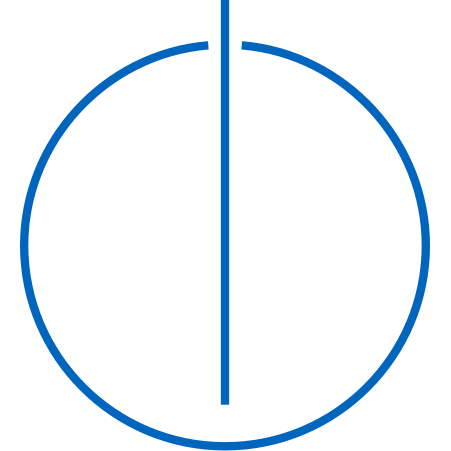
\includegraphics[height=20mm]{logos/faculty.png}
  }{}
\end{titlepage}


\frontmatter{}

\begin{titlepage}
  \centering

  \IfFileExists{logos/tum.pdf}{%
    
\includegraphics[height=20mm]{logos/tum.pdf}
  }{%
    \vspace*{20mm}
  }

  \vspace{5mm}
  {\huge\MakeUppercase{\getFaculty{}}}\\

  \vspace{5mm}
  {\large\MakeUppercase{\getUniversity{}}}\\

  \vspace{20mm}
  {\Large \getDoctype{}}

  \makeatletter
  \vspace{15mm}
  \ifthenelse{\pdf@strcmp{\languagename}{english}=0}
  {
  {\huge\bfseries \getTitle{}}

  \vspace{10mm}
  {\huge\bfseries {\getTitleGer{}}}
  }
  {
  {\huge\bfseries \getTitleGer{}}

  \vspace{10mm}
  {\huge\bfseries \getTitle{}}}
  \makeatother

  \vspace{15mm}
  \begin{tabular}{l l}
    Author:          & \getAuthor{} \\
    Supervisor:      & \getSupervisor{} \\
    Advisor:         & \getAdvisor{} \\
    Submission Date: & \getSubmissionDate{} \\
  \end{tabular}

  \IfFileExists{logos/faculty.png}{%
    \vfill{}
    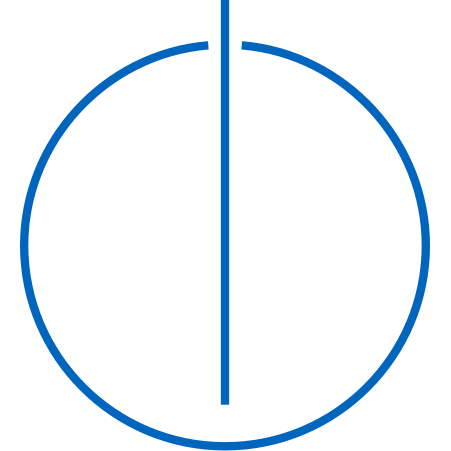
\includegraphics[height=20mm]{logos/faculty.png}
  }{}
\end{titlepage}

\cleardoublepage{}

\thispagestyle{empty}
\vspace*{0.8\textheight}
\noindent
\makeatletter
\ifthenelse{\pdf@strcmp{\languagename}{english}=0}
{I confirm that this \MakeLowercase{\getDoctype{}} is my own work and I have documented all sources and material used.}
{Ich versichere, dass ich diese \getDoctype{} selbstständig verfasst und nur die angegebenen Quellen und Hilfsmittel verwendet habe.}
\makeatother

\vspace{15mm}
\noindent
\getSubmissionLocation{}, \getSubmissionDate{} \hspace{50mm} \getAuthor{}

\cleardoublepage{}

\makeatletter
\ifthenelse{\pdf@strcmp{\languagename}{english}=0}
{\addcontentsline{toc}{chapter}{Acknowledgments}}
{\addcontentsline{toc}{chapter}{Danksagungen}}
\makeatother
\thispagestyle{empty}

\vspace*{20mm}

\begin{center}
\makeatletter
\ifthenelse{\pdf@strcmp{\languagename}{english}=0}
{\usekomafont{section} Acknowledgments}
{\usekomafont{section} Danksagungen}
\makeatother
\end{center}

\vspace{10mm}

Firstly, I would like to thank Prof. Tobias Nipkow, who gave me the opportunity to work on this work 
and introduced Isabelle to me. Then, I want to thank my advisor, Katharina Kreuzer,
for all the meaningful instructions and dedicated guidance she offered. 
It has been a great pleasure to work with her. 
I also want to thank Simon Rosskopf and Kevin Kappelmann, who more or less helped in finding this topic 
and gave some helpful advices about the ongoing project. \\\\
Additionally, I want to thank my parents for their support of my studies in Germany. 
I also want to thank my brother Zichun for sample reading this thesis and providing some insights 
from the perspective of a mathematician. 

\cleardoublepage{}
 % TODO: if you don't have anyone to thank for or don't wish to publish it, comment this line out.
\newcommand{\abstractname}{Abstract}


\chapter{\abstractname}
NP-hardness is a fundamental concept in the complexity theory. It represents a class of problems that 
are hard to be computed by a polynomial-time algorithm. Polynomial-time reductions are used 
to classify the NP-hardness of such problems. While proofs of the correctness of the polynomial-time reductions 
were limited to pen-and-paper proofs, 
it is now possible to reproduce and verify these proofs with the aid of computers. 
There has been an on-going effort to formalise and verify the classical NP-hard problems, 
domonstrating capability of the interactive theorem prover Isabelle in verifying NP-hardness.
On the basis of this effort, we continue to verify the NP-hardness of six problems, 
including Exact Cover, Exact Hitting Set, Subset Sum, Partition, Knapsack, and Zero-One Integer Programming.
\microtypesetup{protrusion=false}
\tableofcontents{}
\microtypesetup{protrusion=true}

\mainmatter{}

\chapter{Introduction}\label{chapter:introduction}
\section{Motivations}
We may encounter many real-life problems that require a decision process to find a solution. 
For example, we always want to choose the shortest queue when shopping at a supermarket. 
Another example is Seven Bridges of Königsberg---is there a way to go through all seven bridges 
without visiting a bridge twice? These problems are formally defined as decision problems.\\\\
NP-hard problems is one of the most famous decision problem classes.
NP-hard problems are hard to be computed by a polynomial-time algorithm. Choosing the shortest queue, 
known as scheduling, is a well-known example for NP-hard problems. There also many other real-life examples
such as map colouring and sudoko.
NP-hardness has been a fundamental research topic in theoretical computer science since the 1970s
when the first few results in NP-hardness were given by Cook \cite{cook2023complexity}, Levin \cite{levin1973universal} 
and Karp \cite{karp2010reducibility}. 
In the next few decades, many attempts were made to show whether NP-hard problems can be computed by a polynomial-time algorithm and to develop approximation algorithms that compute NP-hard problems optimally. 
Among many fields related to NP-hardness, we focus on the polynomial-time reductions, which show the NP-hardness of decision problems. \\\\
All the existing proofs of the correctness of polynomial-time reductions were pen-and-paper proofs, 
which lack automated verification by a computer. 
While human researchers may make mistakes in a proof, the computers are accurate once the system is correctly defined. In addition, 
it is also interesting to show that the computers are able to verify the first few theories that are highly related modern computers today.
With the help of interactive theorem provers, 
it is possible to formalise and verify the classical results of NP-hardness on a computer.
In this manner, we contribute to the theoretical basis of many existing formalisation results, 
e.g. cryptography and approximation algorithms. \\\\ 
There has been an attempt, known as the Karp21 project \cite{polyred}, to formalise NP-hard problems in Karp's paper in 1972 \cite{karp2010reducibility}. 
Our work benefits from this attempt and continues to formalise some of the remaining problems in Karp's paper 
with the interactive theorem prover Isabelle. 

\section{Contributions}
Our work contains two categories of problems. 
\begin{enumerate}
    \item Set covering problems: Exact Cover, Exact Hitting Set
    \item Weighted sum problems: Subset sum, Partition, Knapsack, Zero-One Integer Programming
\end{enumerate}
Set covering problems are problems in which we search for a cover of a given set. In weighted sum problems, 
we look for a set of instances such that their weighted sum reaches another constant bound. While they are the basis of further reductions to problems like 
scheduling, neither of the categories was formalised and verified in the existing project. 
Thus, we chose these problems to complete the project and prepare for potential work in the future.\\\\ 
For each listed problem, we present a polynomial-time reduction either from Satisfiability or another problem listed above. 
Thus, a trace of reductions from Satisfiability can be witnessed. 
Furthermore, proofs of the soundness, completeness, 
and the polynomial-time complexity of each polynomial-time reduction is also presented. \\\\
On the basis of our contribution, it is possible to construct and formalise polynomial-time reduction to other NP-hard problems. 
Additionally, it also provides the theoretical background for other formalisation works related to complexity theory, e.g. 
approximation algorithms, combinatorical optimization etc. 

\section{Outline}
In Chapter 2, we introduce Isabelle dependencies and mathematical backgrounds.\\\\
Chapter 3 and Chapter 4 follow with the formalisation and verification of the listed problems. For each decision problem, 
we define the problem and the reduction. Then, we sketch the proof of the correctness of the reduction and the polynomial-time complexity.
Finally, we present a few concrete implementation details. Examples are also offered for reductions that are rather complicated. 
In Chapter 3, we discuss the polynomial-time reduction of the set cover problems, while Chapter 4 consists of the weighted sum problems. \\\\
To finish, we conclude the current status of the Karp21 project
and present a few possibilities for verifying the rest of the problems in Chapter 5.

\newcommand{\red}{\leq_p}
\newcommand{\problem}[3]{
\begin{definition}
    {#1} \\
    \textbf{Input}: {#2}\\
    \textbf{Output}: {#3}
\end{definition}
}
\newcommand{\bigO}[1]{$\mathcal{O}({#1})$}

\chapter{Preliminaries}\label{chapter:preliminaries}
\section{Isabelle and Dependencies}
\subsection*{Isabelle/HOL}
Isabelle is a generic interactive theorem prover. HOL is the Isabelle's formalization of Higher-Order Logic, a logical system with inductive sets, types , well-founded recursion etc. Our implementation requires the introduction of new datatypes, formalisation of natural numbers and integers. Thus, this type system is necessary.


\subsection*{HOL-Real\_Asymp and Laudau\_Symbols}
TODO

\subsection*{NREST}
TODO

\subsection*{The Karp21 Project}
The project aims to formalise all of the 21 \NPH\ problems in Karp's paper in 1972. Up till now, there are \textbf{TOCOUNT} problems of them finished, with a few other \NPH\ problems that are related but not in Karp's list. Our work also contributes to this project, formalising six of the remaining problems. Though dependent on this project, our work only reuses a few definitions by the predecessors, while the most formalisation and verification is original. An overview of the project is given in the following graph.
\begin{figure}[h!]
\centering
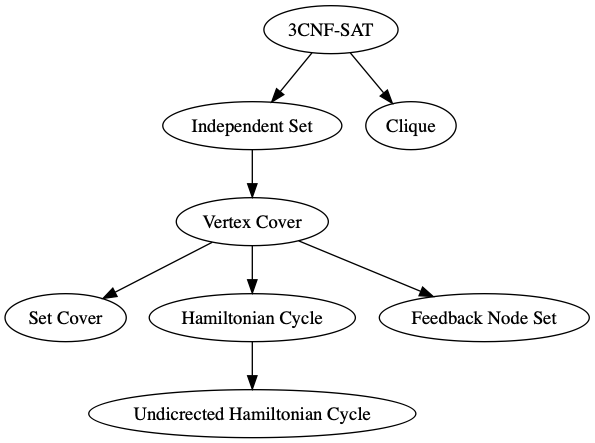
\includegraphics[scale=0.4]{figures/reductions.png}
\caption{Name}
\end{figure}

\subsection*{DigitsInBase}
This entry of Archive of Formal Proofs shows the uniqueness of representation of natural numbers given an arbitrary base. In other words, it proves the well-definedness of the n-ary counting systems. Our implementation benefits from this repository in showing the correctness of the polynomial reduction from \XC\ to \Part.

\section{NP-Hardness and polynomial reductions}
\subsection{Asymptotic Notation}
Conventionally, the asymptotic notation is used for defining complexity classes and for performing the algorithm analysis. 
We follow this convention and choose the big $\mathcal{O}$ notation for algorithm analysis. To begin with, we present a brief
introduction to the asymptotic notation.
\begin{definition}
    Let $f: \mathbb{R} \rightarrow \mathbb{R}$, $g: \mathbb{R} \rightarrow \mathbb{R}$ be two real valued functions with the same domain. 
    $f(x)$ is big $\mathcal{O}$ of $g(x)$, which writes
    \begin{align*}
        f(x) \in \mathcal{O}(g(x))
    \end{align*}
    if there exists a real $M \geq 0$ and a real $x_0$ s.t. 
    \begin{align*}
        |f(x)| \leq M |g(x)|, \forall x \geq x_0
    \end{align*}
\end{definition}
Thus, $f$ is above bounded by $g$. In other words, $f$ is utmost as complex as $g$. Following this definition 
we can derive many complexity classes by $g$. A short list of commonly encountered complexity classes is given 
in table.
\begin{table}[H]
    \centering 
    \begin{tabular}{|| c | c | c ||}
        \hline 
        Name & Big $\mathcal{O}$ Notation & Algorithmic Examples \\ 
        \hline 
        Constant & $\mathcal{O}(1)$ & Parity check\\
        \hline 
        Logarithmic & $\mathcal{O}(\log n)$ & Binary search in a sorted array \\ 
        \hline 
        Linear & $\mathcal{O}(n)$ & Addition of integers \\
        \hline 
        Quasilinear & $\mathcal{O}(n\log n)$ & Merge-sort and heap-sort \\
        \hline 
        Polynomial & $\mathcal{O} (n^c), c \in \mathbb{N}$ & Matrix multiplication \\
        \hline 
        Factorial & $\mathcal{O} (n!)$ & Enumeration of partitions of a set\\
        \hline 
    \end{tabular}
    \caption{List of commonly encountered complexity classes.}
\end{table}

In most cases of this paper, we only consider the polynomial class, which contains the most classes listed above 
as subclasses except for the factorial class. For the purpose of simplicity, we did not 
formalise the theory of asymptotic classes and big $\mathcal{O}$ notation, but used the 
available \textsc{Isabelle} dependencies of \textbf{HOL-Real\_Asymp} and \textbf{Landau\_Symbols}.

\subsection{Decision problems}
\begin{definition}
    A decision problem is a yes-no question on an infinite set of fixed type of inputs.
\end{definition}
Generally, if we refer to a decision problem $A$, we are referring to the set of all inputs for which the answer to the yes-no question is yes. 
The handling of a decision problem usually involves two questions:
\begin{enumerate}
    \item Is there an algorithm, which computes the solution to this problem, terminating on all inputs?
    \item If the answer to the first question is yes, is this algorithm efficient?
\end{enumerate}
If the answer to the first question is yes for a problem, it is a decidable problem, otherwise it is non-decidable. 
We do not expect a yes or no answer for the second question, but would like to find 
the optimal complexity for the algorithm. While some problems are possible to computed in 
an optimal upperbound by a deterministic algorithm, there are also a few problems, for which 
no deterministic polynomial algorithm is found. We define them formally as \NP.
\begin{definition}
    If there is a non-deterministic algorithm 
    that decides the solution to the problem in polynomial time, it is in the complexity 
    class \NP. 
\end{definition}
\begin{definition}
If a problem is at least as complex as the most complex problems in \NP. It is 
    in the complexity class \NPH.
\end{definition}

Although many attempts have benn made to prove or reject the existence of a non-deterministic algorithm 
for the \NP\ problems, our work focuses on the NP-Hardness. We would like to formally prove 
that many classical decision problems are \NPH. For this reason, we have to introduce polynomial reduction.

\subsection{Polynomial reductions}
Given two decision problems $A$ and $B$, 
a reduction is a function $f: A \rightarrow B$, 
which maps the inputs of the question of the first problem 
to that of the second problem. A reduction is polynomial 
if and only if the reduction function has a polynomial bound. 
For a polynomial reduction from $A$ to $B$, we writes $A \red B$. \\ \\
Let $M$ and $N$ denotes the domains of $A$ and $B$ respectively. 
A function $g: M \rightarrow N$ is a polynomial reduction 
if and only if the following conditions are fulfilled.
\begin{align}  
    &x \in A \iff g(x) \in B \\
    &\exists k\in \mathbb{N}. f \in \mathcal{O}(n^k)
\end{align}
For the convenience reason, we usually separate (2.1) into the soundness and completeness of the reduction.
\begin{align}
    soundness: \quad x \in A \Longrightarrow g(x) \in B \\
    completeness: \quad g(x) \in B \Longrightarrow x \in A
\end{align}

\subsection{NP-Hardness and \SAT}
To show a decision problem $B$ is \NPH, 
we have to find a \NPH\ problem and polynomial reduction 
s.t. $A \red B$. A first proven \NPH\ problem is \SAT, 
which was independently proven by Cook in 1971 and Levin in 1973. 
The \SAT\ problem is denoted by 
\problem{\SAT}{A propositional logical formula in 
conjunctive normal form. }{Is there a valid assignment for this formula?}
In the previous implementation of the project, the \SAT\ is defined by a list of clauses, with the clauses as the sets of variables.
There have been many attempts to solve \SAT\ problem in a polynomial bound, 
as well as many approaches to solve \SAT\ problem efficiently in certain scenarios.
Thus, \SAT\ is one of the most studies \NPH\ problems, from which there are also many \NPH\ problems reduced. 
Our first reduction also stems from \SAT, while all the other reductions are constructed upon novel introduced problems. 
More details on the reduction and implementation are given in Chapter 3 and Chapter 4. A glimpse of the available 
implementation is given by
\Snippet{cnf-sat-def}

\subsection{Application of NREST and paradigm}
The NREST package offers an approach for approximating the complexity of non-deterministic processes.
This is especially useful when iterating a set, a collection or any other unordered data structures. Thus,
we use this package throughout this work. In our complexity analysis, the following commands are used. 
\begin{itemize}
    \item \textbf{$RETURNT$ res}. A command that returns the result \textbf{res}. It costs exactly one time unit.
    \item \textbf{$SPECT$ [cond $\rightarrow$ cost]}. A command used for checking a condition. Checking the condition \textbf{cond}
    take \textbf{cost} time units.
    \item \textbf{$SPEC$ $P$ $Q$}. A command used for assignment. Should $P\ x$ hold for an object $x$, it is a valid object after the assignment,
    which takes $Q\ x$ time units.
\end{itemize}
To apply the NREST approach in the complexity analysis, we convert the algorithm into the NREST commands.
During the conversion, we follow the following principles for counting the complexity.
\begin{enumerate}
    \item Checking the condition always costs only time unit. 
    \item Per iteration it costs 1 time unit each for iteration, modification and insertion.
    \item All other operations costs should cost one time unit, if not stated explicitly.
\end{enumerate}
Then, it is possible show a few property of this approach. 
Let $f$ denote a polynomial reduction from $A$ to $B$, while $f_{alg}$ denotes the NREST version of the reduction.
Furthermore, we define sizing functions $s_A$ and $s_B$ as metrics for the asymptotic classes.
To show that the reduction is polynomial, we show that the reduction is polynomially bounded in terms 
of time and space,which are respectively the \textit{refines} and the \textit{size} lemma.
\begin{align}
    refines: \quad f_{alg}(A) \leq \mathcal{O}((s_A(A))^k) \\
    size: \quad s_B (f(A)) \leq \mathcal{O}((s_A(A))^k)
\end{align}
In the end, we can conclude the following implementation paradigm to show that a reduction is correct and polynomial.
\begin{enumerate}
    \item Prove that the reduction is correct.
    \item Implement the reduction in NREST commands.
    \item Prove that the reduction costs polynomial time.
    \item Prove that the algorithm costs polynomial space.
\end{enumerate}

\chapter{Set Covering Problems}\label{chapter:covering}
In this chapter, we discuss about the NP-hardness of a few set covering problems. 
Covering problems ask whether a certain combinatorical structure $A$ covers another structure $B$. 
Alternatively, it may also ask for the minimal size of $A$ to cover $B$. 
We focus on a subclass of covering problems, the exact covering problem. In this subclass, 
$A$ covers $B$ exactly, i.e. no element in $B$ is covered twice in $A$. 
In Karp's paper in 1972, the following covering problems were included: Exact Cover, Exact Hitting Set,
3-Dimensional Matching, and Steiner Tree. In our implementation, we reduced Satisfiability to Exact Cover, and then reduced Exact Cover to Exact Hitting Set. 

\section{Exact Cover}
The Exact Cover problem is a special case of the Set Cover. In Exact Cover, it not only looks for a cover, but also requires the existence of 
cover elements to be unique. 
\problem{Exact Cover}{A set $X$ and a collection $S$ of subsets of $X$.}{Is there a disjoint subset $S'$ of $S$ s.t. 
each element in $X$ is contained in one of the elements of $S'$?}
\Snippet{exact-cover-def}

\subsection{Choice of reduction}
Since Exact Cover is a fundamental NP-hard problem, there are many different reductions available. 
Karp's reduction is based on the  Chromatic Number problem. 
Although the Chromatic Number problem was formalised in Karp's 21 project, we did not choose this reduction
because of the complexity of the graph traversal and the differences between Karp's definition and the available Isabelle's definition. 
In the available definition of Chromatic Number, the Chromatic Number $k$ is limited to be at least three. Since 
the Chromatic Number is in \textbf{P} in the case $k = 2$, the alternative definition is correct. However, this raises the difficulty of performing 
a reduction, for it is necessary to consider a special case for $k = 2$. 
On the contrary, there is an easy reduction from Satisfiability to Exact Cover. This reduction does not involve graph traversal.
The only technical barrier is the typeless set. While Isabelle only supports typed sets, we resolve this problem
by creating a container type. More details follow in the section \ref*{sec:sat-imp}. 

\subsection{Reduction Details}
Given a propositional logical formula $F$, we index the variables and the clauses and use the following notations.
\begin{enumerate}
    \item $x_i$ denotes the $i$-th variable in the formula with $x_i \in vars\; F$
    \item $c_i$ denotes the $i$-th clause in the formula with $c_i \in F$
    \item $p_{ij}$ denotes the $j$-th position/literal in the $i$-th clause with $p_{ij} \in c_i$
\end{enumerate} 
Then we construct a set $X$ and which contains all 3 different kinds objects. 
\begin{align*}
    X = vars\; F \cup F \cup \bigcup_{c_i \in F} c_i
\end{align*}
Furthermore, we construct $S$, a collection of subsets of $X$. We determine the following subsets
\begin{enumerate}
    \item $\{p_{ij}\}$. The unary set of positions
    \item $\{c_i, p_{ij}\}$. The binary set of a clause and a position in it.
    \item $pos(x_i) := \{x_i\} \cup \{p_{ab} | p_{ab} = x_i\}$. The set of its positive occurrences as positions.
    \item $neg(x_i):= \{x_i\} \cup \{p_{ab} | p_{ab} = \neg x_i\}$. The set of a variable with  its negative occurrences as positions.
\end{enumerate}
$S$ contains all of the four types of subsets.
\begin{align*}
    S =& \{{p_{ij}} | p_{ij} \in c_i, c_i \in F \} 
    \cup \{\{c_i, p_{ij}\} | p_{ij} \in c_i, c_i \in F \} \\
    &\cup \{\{x_i\} \cup \{p_{ij} | p_{ij} \in c_i, c_i \in F\} | x_i \in vars\; F, x_i = p_{ij}\}\\
    &\cup \{\{x_i\} \cup \{p_{ij} | p_{ij} \in c_i, c_i \in F\} | x_i \in vars\; F, \neg x_i = p_{ij}\}
\end{align*}
The pair of $(X, S)$ is the input for the Exact Cover\ problem. 
\begin{lemma}[Soundess]
    Let $F$ be satisfiable. The pair $(X, S)$ is then an instance of the exact cover.
\end{lemma}
Let $\sigma \models F$ be a valid assignment. We construct an exact cover $S' \subseteq S$ of $X$ in the following steps.
\begin{enumerate}
    \item For each $x_i \in vars\; F$, $pos(x)$ is included in $S'$ if $\sigma(pos(x)) \equiv \top$. Otherwise we insert $neg(x)$ into $S'$.
    \item For each $c_i \in F$, we choose the minimal $j$ with $\sigma(p_{ij}) \equiv \top$, and insert $\{c_i, p_{ij}\}$ into $S'$
    \item For each $p_{ij} \in c_i$, if $\sigma(p_{ij}) \equiv \top$ and $\{c_i, p_{ij}\}$ is not in $S'$, the unary set $\{p_{ij}\}$ is included. 
\end{enumerate}
Obviously, each position in $pos(x)$ and $neg(x)$ will be false under the assignment $\sigma$, 
while the positions in the other sets are all true. By design, the positions in the second and the third steps never duplicate. 
Thus, no same position occurs in two different sets in the collection $S'$. 
Furthermore, each clause exists in exactly one set in the second step, which is also the case for the variables in the first step.
Hence $S'$ is disjoint. \\\\
From this fact, we can also conclude that clauses and variables are covered in $S'$. 
Now we only have to show that all the positions are covered. If a position $p_{ij}$ is false under $\sigma$, 
it is covered in the first step. Otherwise it is either covered in the second step or the third step. 
\begin{lemma}[Completeness]
    Let $(X, S)$ be reduced from $F$. If $(X, S)$ is an instance of the exact cover, $F$ has to be satisfiable.
\end{lemma}
Given an exact cover pair $(X, S)$ reduced from $F$, it is easy to reconstruct the model $\sigma$ with the same approach as in the proof of the soundness, 
showing that $F$ is satisfiable. Thus, the completeness of the reduction is proven. 
\begin{lemma}[Polynomial Complexity]
    The construction of $(X, S)$ from $F$ is polynomial. 
\end{lemma}
In the reduction, we have to iterate all of the variables, the clauses and the positions. 
Thus, we have to find a polynomial bound with regards to three metrics. Let $n, m$ and $k$ denotes 
the number of variables, clauses and postitions respectively. To derive the three metrics, we have to iterate 
all of the clauses, resulting the complexity of \bigO{m}. Unexpectedly, this results in the set $X$, 
indicating a linear complexity for the construction. \\\\
Now the interesting part is the collection $S$. For each type of subsets, we give a polynomial bound 
\begin{enumerate}
    \item $\{p_{ij}\}$. It is sufficient to merely iterate the positions, which requires the complexity of $k$.
    \item $\{c_i, p_{ij}\}$. Each clause is iterated for $|c_i|$ times. Since $|c_i|$ is a constant, there is a $c \in \mathbb{N}$ 
    s.t. $|c_i| \leq c$. Obviously, the complexity is above bounded by $c \cdot m$.
    \item $pos(x)$ and $neg(x)$. For each variable $x$, it is required to iterate all of the positions, which produces the complexity 
    of $2 \cdot nk$ in total.
\end{enumerate}
Thus, the construction costs the polynomial complexity of $k + cm + nk \in \mathcal{O}(nk + m)$. 
With the linear complexity of the construction of $X$, we conclude that the reduction has the polynomial complexity.

\subsection{Implementation Details}
\label{sec:sat-imp}
\subsubsection{Reduction and Proof}
Intuitively, the variables, positions and clause can be represented by indices or tuples of indices. However, it it not easy 
to unify the representation s.t. they are of the same type. One possible solution is introducing a new dimension in the tuple, 
and use it to classify the representated objects. However, we might still have to introduce a new enumerate type for this purpose. 
On the contrary, a container type is exempted from the tedious handling of tuples, although it still introduces a new type. Thus, 
we implement this container type with a few auxiliary functions \textbf{xc\_element} as folows. 
\Snippet{exact-cover-basics}
Then, it is possible to define the reduction function. 
\Snippet{exact-cover-red}
Proof of the correctness of the reduction argues about the disjointness and covering property by showing that a specific type of element 
is existent or non-existent in the constructed sets. Though the majority of the proof is lengthy, it does not require too many techniques 
and is overall trivial after applying the corresponding lemmas and definitions.\\\\
The only exception is the construction of $\{c_i, p_{ij}\}$ in the second step. $p_{ij}$ is chosen as the position with the least index. However, 
in our definition, there is no such indexing property in the \textbf{xc\_element} datatype, meaning that such construction is not possible. 
Fortunately, the choice of the $p_{ij}$ does not necessarily require a minimal index. Any arbitrary $p_{ij}$ that is true under the assignment 
$\sigma$ is a valid choice. For this reason, we chose to use the \textbf{SOME} predicate in Isabelle, which obtains an arbitrary instance that fulfills
the required property. 
\Snippet{exact-cover-prf} 
To end with, we show that the reduction is sound, complete, and consequently correct. 
\Snippet{exact-cover-correct}

\subsubsection{Polynomial Complexity}
To begin with, it is necessary to determine to metrics, on which the complexity is dependent. For 
a logical formula $F$, we will iterate all of the variables, clauses and positions. Hence all of them are need for as metrics. 
Nevertheless, the NREST implementation does not support a complexity bound with different metrics. As a result, it is necessary to 
choose the maximum of all metrics and use it as our sole metrics\footnote{A few previous reductions from Satisfiability uses the number of clauses 
as a metrics. It was also corrrect for those reductions iterated only the clauses.}. Similarly, we define $max |X| |S|$ as the metrics 
for the exact cover instance $(X, S)$. Then we can define the NREST algorithm.
\Snippet{exact-cover-poly}  
The proof of the polynomial bound is, however, hardly automated. Part of the reason is that Isabelle fails to find and apply the monotonicity 
of the space function, time function and the cardinality. For this reason, it is necessary to show such relationships. For example, one of them is about the 
cardinality
\Snippet{exact-cover-polyaux}
Finally, we show the \textit{refines} and \textit{size} lemma as well as that the reduction is polynomial.
\Snippet{exact-cover-final}

\section{Exact Hitting Set}
The hitting set problems are variants of the set covering problems. Essentially, they are two different ways 
of viewing the same problem. Just as the hitting set\footnote{Note that the exact hitting set problem was referred to as the hitting set problem in Karp's work, whereas 
it is generalized to be another problem nowadays.} is a variant of the set covering, the exact hitting set is 
a variant of the exact cover. 
\problem{Exact Hitting Set}{A collection of sets $S$}{Is there a finite set $W$ s.t. the intersection of $W$ and 
each element $s \in S$ contains exactly one element?}
\begin{align*}
   \textbf{Exact Hitting Set} := \{S\ |\ \exists W.\ \forall s \in S.\ |W \cap s| = 1\}
\end{align*}
 

\subsection{Reduction Details}
Given an exact cover pair $(X, S)$, the hitting set input $C$ is constructed by 
\begin{align*}
    C = \{\{s | u \in s, s \in S \} | u \in X\}
\end{align*}
Thus, $C$ is the set of sub-collections denoted by $c_u$. All sets in $c_u$ share the same element $u$.
\begin{lemma}[Soundess]
    Let $(X, S)$ be an exact cover instance. A collection $C$ reduced from $(X, S)$ is then an instance of the exact hitting set.
\end{lemma}
The soundness of this reduction is straightforwardly proven with the existence of $S'$ that covers $X$ exactly.
For the soundness of the reduction, it suffices to show 
\begin{align*}
    \exists W.\ \forall c_u \in C.\ |W \cap c_u| = 1
\end{align*}
Let $W = S'$ and $c_u = \{s | u \in s, s \in S \} \in C$ be an arbitrary element. 
Since $S'$ covers $X$ exactly, there is exactly one $s \in S'$ that contains $u$. Moreover, this $s$
is also included in the $c_u$, for $s \in S'$ and $S' \subseteq S$. Thus, it holds that $W \cap c_u = S' \cap c_u = \{s\}$ and consequently $|W \cap c_u| = 1$.
\begin{lemma}[Completeness]
    Let the collection $C$ be a collection reduced from a pair $(X, S)$. If $C$ is an instance of the exact hitting set, 
    $(X, S)$ has to be an instance of the exact cover.
\end{lemma}
The proof of the completeness shares a similar construction. The only difference is that $W$ is not 
necessarily a subset of $S$. Nevertheless, there exists a subset $W' \subseteq W$ s.t. it is not only a subset of $S'$, but it
also fulfills the same property as $W$. Let $S' = W'$, the completeness is then proven analogously as the soundness. 
\begin{lemma}[Polynomial Complexity]
    The construction of $C$ from $(X, S)$ is polynomial. 
\end{lemma}
Finally, we show that the reduction is polynomial. In our reduction, it is necessary to iterate the set $X$ and the collection $S$ in a nested loop. 
With the cardinality $|X|$ and $|S|$ as the metrics, it is obvious that the reduction costs the complexity of \bigO{|X||S|}.

\subsection{Implementation Details}
\subsubsection{Reduction and Proof}
Since the exact cover problem is defined over a finite set $X$ and a finite collection $S$, we have to check if the $X$ and $S$ are finite and 
if $S$ is a collection of $X$. Thus, a condition statement, which checks this requirement, is added to the implementation. Furthermore,
the proof of the correctness is implemented as described above. Following is a snippet of implemented definitions and lemmas.
\Snippet{exact-hitting-set-def}
\Snippet{exact-hitting-set-reduction}

\subsubsection{Polynomial Complexity}
We determine the size of the exact hitting set entry $C$ as $|C|$. According to the paradigm, 
we define the NREST algorithm and show the \textit{refines} and \textit{size} lemma as follows

\Snippet{exact-hitting-set-poly}

The proof of is mostly automated after unfolding the necessary definitions. 
However, an additional step is required for indicating the relationship between the sizing functions. 
While it holds $|C| = |X|$, 
the size of the exact cover is defined by $max |X| |S|$ instead of $|X|$. Hence we can
only conclude that the size of the exact hitting set is less equal than the size of the exact cover. 
The proof automation will then fails in showing $|C| \leq |S| \cdot |S| + 1$ when $|S| \geq |X|$. 
For this reason, we have to prove one additional lemma about the cardinality of the 
exact hitting set.

\Snippet{exact-hitting-set-aux}

Finally, we show that the reduciton is correct and polynomial. 

\Snippet{exact-hitting-set-final}








\appendix{}

% TODO: appendix chapter
\chapter{Examples for reductions}
In this part we present examples for polynomial reductions to assist with the understanding. 
\section{Example for polynomial reduction from Satisfiability To Exact Cover}
\textbf{Input:} A logical formula in conjunctive normal form 
\begin{align*}
    F := (x_1 \lor x_2 \lor \neg x_3) \land (\neg x_1 \lor x_2) \land (x_1 \lor x_3)
\end{align*}
\textbf{Output:}
The constructed set is
\begin{align*}
    X := & \{ x_1 ,x_2, x_3\} \cup \{c_1, c_2, c_3\} \cup 
    \{p_{11}, p_{12}, p_{13}, p_{21}, p_{22}, p_{31}, p_{32}\}
\end{align*}
The constructed collection is 
\begin{align*}
    S : = & \{\{p_{11}\}, \{p_{12}\}, \{p_{13}\}, \{p_{21}\}, \{p_{22}\}, \{p_{31}\}, \{p_{32}\}\} \\
      & \cup  \{\{c_1, p_{11}\}, \{c_1, p_{12}\}, \{c_1, p_{13}\}, \{c_2, p_{21}\}, 
      \{c_3, p_{31}\}, \{c_3, p_{32}\}\} \\ 
      & \cup \{\{x_1, p_{11} p_{31}\}, \{x_1, p_{21}\}, \{x_2, p_{12}, p_{22}\}, \{x_2\},
      \{x_3, p_{32}\}, \{x_3, p_{13}\}\}
\end{align*}
\textbf{Validity:} Apparently, the only valid assignment $\sigma$ of $F$ is given by 
\begin{align*}
    \sigma = \{x_1 \equiv \bot, x_2 \equiv \top, x_3 \equiv \top \}
\end{align*}
Wir construct an exact cover $S'$ by 
\begin{align*}
    S' = \{\{c_1, p_{22}\}, \{c_2, p_{21}\}, \{c_3, p_{32}\},
    \{x_1, p_{11}, p_{31}\}, \{x_2\}, \{x_3, p_{31}\},
    \{p_{22}\}\}
\end{align*}

\section{Example for polynomial reduction from Exact Cover To Subset Sum}
\textbf{Input:} The instance of exact cover is given by 
\begin{align*}
    X &:= \{1, 2, 3, 4\} \\ 
    S &:= \{\{1\}, \{2\}, \{2, 3\}, 
    \{2, 4\}, \{3, 4\}, \{1, 2, 3\}\}
\end{align*}
\textbf{Output:} 
While $S$ is not changed, the weighting function $w$ and the sum $B$ is given by 
\begin{align*}
    w(s) = \sum_{x \in s} 4^x,
    B = w(X) = 4 + 4^2 + 4^3 + 4^4 = 340
\end{align*}
\textbf{Validity:} An exact cover $S'$ is given by 
\begin{align*}
    S' = \{\{1\}, \{2\}, \{3, 4\}\}
\end{align*}
Hence it holds that 
\begin{align*}
    w(\{1\}) + w(\{2\}) + w(\{3,4\}) = 4 + 4^2 + (4^3 + 4^4) = 340 = B
\end{align*}

\section{Example for polynomial reduction from Subset Sum To Partition} 
\textbf{Input:} We use the same subset sum entry as in the previous example. $(S, w, B)$ be 
then converted to 
\begin{align*}
    as &:= [4, 16, 80, 272, 320, 72] \\ 
    s &:= 340
\end{align*}
\textbf{Output:} The reduced $bs$ is then 
\begin{align*}
    bs := [425, 341, 4, 16, 80, 272, 320, 72]
\end{align*}
\textbf{Validity:} With $as' = [4, 16, 320]$, the corresponding $bs'$ is 
\begin{align*}
    bs' = [425, 4, 16, 320] \\ 
    bs - bs' = [341, 80, 272, 72]
\end{align*}
with the equality
\begin{align*}
    425 + 4 + 16 + 320 = 765 = 341 + 80 + 272 + 72 
\end{align*}

The other reductions are easier to understand, hence no example is provided here.



\microtypesetup{protrusion=false}
\listoffigures{}
\listoftables{}
\microtypesetup{protrusion=true}
\printglossaries
\printbibliography{}

\end{document}
